% Formatting for JEcol
\documentclass[12pt]{article}

% amsmath package, useful for mathematical formulas
\usepackage{amsmath}
% amssymb package, useful for mathematical symbols
\usepackage{amssymb}
% graphicx package, useful for including eps and pdf graphics
% include graphics with the com and \includegraphics
\usepackage{graphicx}

% citep package, to clean up citations in the main text. Do not remove.Editor mode.
% Formatting for JEcol

\usepackage{natbib}
\usepackage{booktabs} % To thicken table lines
\usepackage{color} 
\usepackage{multirow}
\usepackage{xcolor} % Required for specifying colors by name
%\definecolor{color}{RGB}{128,0,0} % Define the color used for highlighting throughout the book
\definecolor{color}{RGB}{0,0,0}%{64,63,111} %navy blue % Define the color used for highlighting throughout the book
\definecolor{blue}{RGB}{69,74,159} %Redifines the default for the color blue
\definecolor{niche}{RGB}{128, 20, 17}
\definecolor{neutral}{RGB}{9, 19, 70}
\definecolor{nineu}{RGB}{214, 168, 56}
\definecolor{grey}{RGB}{180,177,172}

\usepackage{makecell} % for cell alignment 

\usepackage{mdframed} % for cell alignment 

% non ascii characters
\usepackage[T1]{fontenc}
\usepackage[utf8]{inputenc}

% Use doublespacing - comment out for single spacing
\usepackage{setspace} 
\doublespacing

% Text layout
\topmargin 0.0cm
\oddsidemargin 0.5cm
\evensidemargin 0.5cm
\textwidth 16cm 
\textheight 21cm

% Bold the 'Fig #' in the caption and separate it with a period
% Captions will be left justified
\usepackage[labelfont=bf,
labelsep=period,justification=raggedright]{caption}
\renewcommand{\figurename}{Figure}

% create command for model formulas
\renewcommand{\Rsquared}{R{$^2$}}
%\renewcommand{{$|$}}{{$|$}}
%\renewcommand{\e}{{$+$}}
%\renewcommand{\int}{{$*$}}

% Leave date blank
\date{}

\pages

\pagestyle{myheadings}
%% ** EDIT HERE **

\usepackage{lineno}
\linenumbers

%% ** EDIT HERE **
%% PLEASE INCLUDE ALL MACROS BELOW

%% END MACROS SECTION

\begin{document}

\begin{flushleft}
{\Large
{\textbf{Tailoring species abundance distributions with
trait-environment correlations
% other suggestions
% Tailoring species abundance distributions to untie niche and neutral processes
}}
}
\end{flushleft}


% abstract 150 words
\section*{Abstract}

%short abstract
%We propose a novel, general test to assess which mechanisms drive SADs. It translates niche and neutral mechanisms into fixed and random effects in a generalized linear mixed model. We applied this methodology to fern metacommunity along an altitudinal gradient. Hypotheses for niche processes, neutral and an hierarchical combination of both were tested. We found that although some ecological strategies confer on average more abundance in a particular altitude, drift results in variance in species abundances within the same ecological strategy. Accordingly, we were able to define ecological strategies in fern community based on synthetic and objective traits, and our modeling approach unpack neutrality in drift and limited dispersal mechanisms. Furthermore, predictions from our model fit SADs on each altitude. By adding information of species traits we did not reject the idea of functional equivalence of species, we delimited the influence of neutral processes on community assembly and SADs. 

% long abstract: 
%The pattern of few abundant and several rare species is considered a general law in ecology. Since both niche and neutral models can explain species abundances distributions (SADs), incorporating species differences in relation to its traits can help us understand to what extent functional divergence and equivalence can affect SADs. We used a trait-environment approach to understand which ecological strategies of species, if any, affect SADs in a fern metacommunity along three mountain ranges in a Brazilian Atlantic rainforest. We tested hypothesis simultaneously for purely neutral, purely niche and an hiearchical combination of both processes (emergent group, i.e. combination of groups of species defined by functional divergence that within behave as functional equivalents). We built statistical models using generalized linear mixed models (glmm) to represent our hypothesis. Our framework is based on the idea that we can translate neutral and niche processes into random and fixed effects in glmm's. We modeled the effect of dispersal limitation and drift within species sharing the same ecological stategy as random effects and used fixed effects to represent niche influences due to species ecological strategies and the altitudinal gradient. We found that species abundances are defined by a hierarchical combination of niche and neutral processes. We identified that combination of different states of laminar thickness and life form defines an ecological strategy and the emergent group. Although some ecological strategies are related to high abundance values in a particular altitudinal level, we still found a variance component in abundance among fern species sharing the same ecological strategy. Variance was explained by random effects representing functional equivalence within species sharing the same ecological strategy and limited dispersal among altitudinal levels and mountain ranges. Tradeoffs of an ecological startegy with its position on the gradient are due to strategies for reducing water loss across the altitudinal gradient. Additionally, we found that abundance predicted by our model fits perfectly with SADs on each altitudinal level. Finally, on the niche side, we defined ecological strategies in fern community based on synthetic and objective traits. On the neutral side, our modelling approach unpack neutrality in drift and limited dispersal mechanisms. By adding information of species traits we do not rejected the idea of functional equivalence of species, we refined the scope of the effect of neutral processes in terms of drift within emergent groups and limited dispersal.

%JEcol abstract

1. Given that both niche and neutral models can explain species abundances distributions (SADs), incorporating species differences in relation to its traits can help us understand to what extent functional divergence and equivalence can affect SADs. We proposed a trait-environment approach to understand which ecological strategies of species, if any, affect SADs at metacommunities across environmental gradients. 

2. We propose a straightforward framework to simultaneously test hypotheses for purely neutral, purely niche and and a combination of both processes (i.e. combinations of groups of species that are functionally divergent across groups but neutral within the group). This framework combines functional traits with generalized linear mixed models (GLMMs) to represent the niche and neutral processes. Specifically, we show how to translate neutral and niche processes into random and fixed effects in GLMM's. We apply our framework for core and occasional species separately in a fern metacommunity. %For neutral processes we show how our framework can separate dispersal limitation and drift.

3. We used this framework to understand how niche and neutral processes affect SADs in a fern metacommunity along three mountain ranges in a Brazilian Atlantic rainforest. We found that for core species a a hierarchical combination of niche and neutral processes best explained the data. Differently, occasional species are driven by neutral processes only. % 
For core species, different combinations of laminar thickness and life form define distinct ecological strategies. Specific ecological strategies determined high abundances at a given latitude, consistent with the idea of ecological filtering, but we also found a variance component in abundance among fern species sharing the same ecological strategy. This variance in abundance within a group was explained by a combination of drift and dispersal limitation. Tradeoffs of an ecological strategy with its position on the gradient are due to strategies for reducing water loss across the altitudinal gradient.

4. As demonstrated by our example, our framework has the potential to quantify the relative importance of different processes (niches/filtering, drift, and dispersal limitation) from spatially structured abundance and functional trait data. Additionally, our framework allowed us not only to rebuild SADs curves for local communities, but also to provide a mechanistic explanation for species abundance patterns. 

%Tweetable abstract
%We present a framework to tailor species abundances in local communities by untying the effect of niche and neutral process.

%We present a simple linear modeling framework to reveal the influence of niche and neutrality on community assembly. Besides its generality, our framework shows quantitatively the influence of both processes. 

{\bf Keywords}: emergent groups, drift, fern communities, functional groups, limited dispersal, neutrality, niche, SADs.

\newpage

\section*{Introduction}
% precisa incluir o que ter Braak e Jamil tem feito, 
% incluir também Miller 2019 e Ovaskainen 

Most species abundance distributions (SADs) in biological communities can be explained equally well by niche and neutral mechanisms \citep{McGill2007}. 
In this case, the problem of distinct processes explaining the same pattern seems to be related to the fact that SADs do not use species identities, which is indeed consistent with the idea of ecological equivalence in neutral theory. Ecological equivalence implies that trophically similar species are demographically identical \citep{Hubbell2001, Hubbell2005}. Therefore, differences in species abundances should be a result of random birth and death events at the local scale that make communities diverge by drift if dispersion is limited \citep{Hubbell2001, Hubbell2005}. 
In contrast with this neutral view, species identities would matter if the lineages evolved a distinctive set of adaptive traits that translate into different niches. In this case, species traits should correlate with abundances, and thus one way to distinguish between neutral and niche processes on SADs would be to assess such correlations. 
If the ecological equivalence hypothesis is rejected, a strong theory for SADs would be the one that could predict not only the shape of the curve but also if a species would be common or rare based on its traits \citep{Mcgill2003}. 
For instance, SADs have been described as a mixture of abundances of two groups of species, the core (persistent) and satellite (occasional) species \citep{Magurran2003}.
% PI ter 13 out 2020 09:37:50 -03: Sugestão "Moreover, sets of species can be more or less ecological equivalent, and thus SADs can be a mixture ...
% PI 17 dez 2020: sugeri est iníco de sentença acima pq acho que o "for instance" está fazendo uma passagem meio brusca de aum assunto ao outro. Se não for isto acho que precisa conectar melhor com o as sentenças anteriores de algum jeito.
Core and occasional species would follow different statistical models for SADs, indicating that these two groups are being affected by different processes. Furthermore, \cite{Supp2015} showed that core and satellite species exhibit different life-history strategies, showing a link between temporal persistence, local abundance and species life-history traits.

The recognition of different groups of species in the local community is an important step to put SADs in a broader ecological and evolutionary context \citep{McGill2007, Swenson2012}, but we can go further by asking what defines each group. The obvious choice to identify groups of species in SADs is to look for traits that correlate with their abundances.  Thus, placing SADs in a framework that allows testing the ecological equivalence of species would help to disentangle underlying niche and neutral mechanisms. Assessing trait-environment correlations in community ecology has concerned ecologists for decades since \cite{Raunkiaer1934} characterization of plant life forms adapted to the environment \citep[see also][]{Grime1977, Connell1978}. Early development of a trait-based approach focused on descriptions of the variation of life history traits along environmental gradients. In the past 20 years, trait-based approaches focused on quantitative measurements of traits for testing non-random trait dispersion in community assembly
\citep{Swenson2012}. The redefinition of the niche concept \citep{Chase2003},
%PI ter 13 out 2020 09:42:29 -03 : Eu diria "the refinig of the niche concept" ou recent developments in the niche concept. Acho que o Chase & Leibold não trazem tanta novidade assim em relação ao Tilman e mesmo o Hutchison.
modern coexistence theory \citep{Chesson2000}, and Hubbell's proposal of neutral theory \citep{Hubbell2001} contributed to
%the bloom of functional ecology as a test against neutral theories.
advance functional ecology as alternative framework to neutral theories. 
Empirical and theoretical tests in the context of functional ecology have been followed by a massive analytical development \citep{Kraft2010} from basic functional diversity measures
\citep{Petchey2002a, Petchey2007} to different approaches for incorporating functional evenness and divergence \citep{Mason2005, Pavoine2009} and multi-trait analysis \citep{Laliberte2010}, patterns of niche overlap \citep{Mason2008}, mechanisms of environmental filtering \citep{Kraft2007, Mayfield2009}, and trait
variation across environmental gradients \citep{shipley2006plant, cornwell2009community, messier2010traits}. 
The remarkable influence of trait-based approaches in plant community ecology could be considered a paradigm shift from species to trait-based ecology \citep{Pavoine2011, Swenson2012}, represented by the emergence of methods and theories as well as the implementation of a global database for plant species traits (TRY) \citep{Kattage2011}.
% adicionando aqui info da Jamil e ter Braak. Precisa contextualizar trait-environment models Miler and Ovaskainen
In addition, a few multilevel model approaches \citep{Pollock2012, Jamil2013, Jamil2013a, Miller2019, TerBraak2019} have been developed to assess trait-environment models from community data. Differently from the emphasis in quantifying diversity through metrics, these models allow to detect what drives species abundance in a community.
%PI ter 13 out 2020 09:49:45 -03: acho que aqui pdoeria já ser mais específico sobre o que esta abordagem faz. Algo como "Differently from the emphasis in quantifying diversity through community-wide metrics, these models relates the abundances of each species to their traits.
Still, much of this trait-based work has focused on species interactions independent of SADs \citep{Swenson2012}. 
Even thought here have been some efforts to incorporate trait information in SADs \citep{Magurran2003, Supp2015} by asking what defines functional groups we can go further by asking what is the relative importance of biological traits versus stochasticity in shaping species abundances.
%PI ter 13 out 2020 09:52:49 -03: acho que o trabalho do Ter Braak e talvez boa parte do Joint-sepcies models tb façam parte deste esforço. Aí acho que já não caracterizaria "some efforts", pq é bastante coisa. Talvez indicar que a abordagem da Magurram e estes modelos vão na direção de incorporar traits na análise de SADs e com isso reconhecer diferentes grupos funcionais e que isso por sua vez pode ajudar a investigar the relative importance of biological traits versus stochasticity in shaping species abundances.

 
There is an emerging consensus that both niche and neutral dynamics are important for community assembly \citep{Vellend2014} and that community ecology should answer how the two processes operate together \citep{Gravel2006, Herault2007, Ovaskainen2017}. Overcoming the dichotomy debate of niche versus neutrality, Vellend proposes that biological communities are affected by the big four high level processes defining biological communities (i.e. selection, drift, speciation and dispersal). In this context, niche and neutral dynamics %are under the umbrella of
corresponds to
selection and drift. Therefore, the debate is now focused on how to disentangle and quantify the influence of different processes. % cite Vellend 2010 and book %PI ter 13 out 2020 09:57:45 -03: achei que esta sentença repete o que já foi dito, que está claro já.

One way of combining drift and selection dynamics is through the delimitation 
of the set of species in which neutrality applies \citep{Tilman2004, Scheffer2006, Herault2007, Holt2007}. Emergent Groups are defined as sets of species in a local community which are functionally similar enough with each other that their dynamics are well approximated by drift processes \citep{Herault2007}. Thus, selection through niche differentiation defines each Emergent Group, and within the Emergent Group drift defines species abundances in the local community. The Emergent Group approach represents the scenario in which neutral and niche dynamics operate at different levels generating SADs. %Herein,we
We built on this idea to
propose a framework to quantify the influence of selection and drift dynamics at local and regional scale based on trait-environment correlations. Our framework puts a multilevel model approach \citep{Pollock2012, Jamil2013, Jamil2013a, Miller2019, TerBraak2019} 
in the context of niche and neutral dynamics to describe SADs. 

Our main goal is to test which combination of mechanisms drives species abundance in local communities along environmental gradients. We used as a study system metacommunities of ferns across an altitudinal gradient sampled in three localities. 
We start from three potential mechanisms that can explain SADs: (i) purely drift,  (ii) purely selection, (iii) the integration of both with the Emergent Group approach, and derived four hypotheses. %Given
Assuming
that SADs contain core and satellite species and these groups seem to present different patterns of SAD, we aimed to test our hypotheses for the two groups separately. 
The first hypothesis is that drift dynamics are dominant and species abundances vary among communities
%PI ter 13 out 2020 10:10:59 -03 among communities ou among core and transient groups? Enfim, não precisa incluir nas hipóteses explicitamente estes grupos?
randomly, as a result of drift under limited dispersal.
Our second hypothesis is that selection dynamics are dominant and species abundances are determined by a set of adaptive traits, herein named ecological strategy. 
In this case, species abundance in the local community would be a result of dissimilarities in ecological strategies of species and the optimal strategy would vary along the environmental gradient. 
Third, species abundance are defined by a combination of selection and drift dynamics through Emergent Groups. In the third scenario, ecological strategies of species affect abundance but ecological drift and limited dispersal ensues random differences of species abundances within each group. As in the niche scenario, the success of the ecological strategies would depend on the environment.
%Fourth, assuming that neutrality effects can appear not only as drift within Emergent Groups, we hypothesize that processes generating Emergent Groups could occur combined with limited dispersal. 
Fourth, our null hypothesis, herein defined as idiosyncratic, postulates that species abundance is a result of random variation among species and sites independently of drift and limited dispersal.
We show how these hypotheses can be translated into fixed and random effects in linear mixed models and tested simultaneously using a model selection framework.
%We thus propose a novel approach that uses random structure of mixed models to represent drift and limited dispersal in the hypotheses where neutrality operates. 
Our proposal is to test what drives species abundance of core and occasional species with our modeling framework and to quantify the relative importance of selection and drift by applying the coefficient of determination R{$^2$} \citep{Nakagawa2013, Nakagawa2017} to the models. The models in our framework were build based on previous trait-correlation approaches \citep{Pollock2012, Jamil2013, Jamil2013a, Miller2019, TerBraak2019}, with the novelty of putting them in the context of selection and drift dynamics and relating them with SADs.
%PI ter 13 out 2020 10:20:32 -03 : achei esta parte final puxando demais para métodos. Vamos pensar em uma formulação que preserve a informação essencial de que há hipóteses altermativas combinadas com variância explicada, sem entrar tanto em detalhes técnicos, ficando só nos conceitos mesmo.


\section*{Material and methods}

\subsection*{Study site and sampling methods}
In order to test for trait-environment correlations on species
abundances we used abundance data of fern species sampled along an
altitudinal gradient in three locations of the Brazilian Atlantic
rainforest at Serra do Mar mountain chain, in Paran\'a State from
\cite{Paciencia2008}.  The sampled gradient ranged from sand dune
vegetation at the coastal plain (0 to 10 m a.s.l.) to high montane
Ombrophilous Forest areas (1,500 m a.s.l.) in three mountain ranges in
this ecorregion: Serra da Graciosa (25{$^{\circ}$} 21'S,
48{$^{\circ}$} 54'W), Pico do Marumbi (25{$^{\circ}$} 27'S,
48{$^{\circ}$} 55'W), and Serra da Prata (25{$^{\circ}$} 37'S,
48{$^{\circ}$} 41'W). From 0 to 700 m a.s.l. the climate is
subtropical with hot summer and without a dry season (Cfa) and with
mean temperature during summer above 22{$^{\circ}$} C. Above 700 m
a.s.l. the climate is subtropical with warm summer and without dry
season (Cfb). Since all mountains are part of the same mountain chain,
with controlled distance (from 14 to 41 km distant from each other),
% PI 17 dez 2020: não entendi o que seria controlled distance. Pequenas o suficiente?
we considered sampling sites at the same altitudinal level as
replicates from local communities.  In fact, floristic similarity
among sites at the same altitude in this mountain chain is higher than
floristic similarity among sites from the same mountain range
\citep{Paciencia2008}.
 
Vegetation along the altitudinal gradient varies following changes in
soil, humidity, temperature, and precipitation levels.  The coastal
plain is occupied by scrubland and low forest on poor, white-sand
soils.  Lowland Ombrophilous Forest occupies the transition between
the coastal plain and the mountain range, where the sandy soil has
poor drainage but higher fertility.  Submontane Ombrophilous Forest
occurs from 30 to 400 m a.s.l. and harbors large trees growing on deep
clay soils of the hillside. Montane Ombrophilous Forest occurs from
400 to 1,000 m a.s.l. on lithic soils limiting the growth of large
trees. Montane forests occur where there are less severe environmental
conditions in terms of humidity, temperature, and
precipitation. High-montane Ombrophilous Forests occurs from 1,000 to
1,600 m a.s.l. with predominance of lithic soils and where woody
stractum is composed by crooked trunks of small size.  We used
elevation above sea level to represent the altitudinal gradient as a
proxy for variation in vegetation type, humidity, temperature, and
precipitation.  Although altitude represents a set of variables, it is
recognized that fern species have specific elevational distributions
related to their ecological requirements \citep{Mehltreter2010} and
fern diversity is correlated with elevation exhibiting a peak at
intermediate elevations
\citep{Kessler2001,Cardelus2006,WatkinsJr2006}.

A total of 30 sites were sampled, 10 in each mountain range %locality,
distributed at 0, 10, 50 m, and from 200 to 1,400 at 200 m elevation
intervals. In each site, one 20 x 20 m plot was
located. % PI 17 dez 2020: randomly located?
All fern individuals under 2 m from the forest floor
% PI 17 dez 2020: não entendi aqui se under 2m from forest floor
% significa até 2 m de altura apenas? Se é isso só não tinha me
% tocado, pq há epífitas tb e achei que a amostragem cobria altura
% maiores
within the plots were recorded %sampled,
including terrestrial ferns, such as terrestrial herbs and tree ferns,
hemiepiphyte and epiphyte herbs (only individuals in which the
lowermost leaf was up to 2 m from the ground).
% PI 17 dez 2020: não seria melhor "all individuals that had at at least one leaf below 2m from the ground"?
Abundance was measured
as the number of ramets of each species in each plot %sample unit.
%The study of Paciencia (2008) recorded 19,938 individuals belonging to 153 fern species.
A total of 19,938 individuals belonging to 153 fern species has been recorded in the plots \cite{Paciencia2008}.

\subsection*{Ecological strategy and species abundances}

In order to assess trait-environment correlations with species
abundances we tested which set of traits define an ecological
strategy. We chose three traits that are related to species local
abundances and that should respond to environmental changes along the
altitudinal gradient.  Our choice was based on limitations imposed on
ferns due to aspects of their biology such as intolerance to
fluctuating conditions and poorly controlled evaporative control
\citep{Page2002}. Ferns may be less efficient in water use than seed
plants due to an inefficient stomatal control, that relies only on
passive closure \citep{Brodribb2011}.  In the absence of strategies to
deal with such limitations, ferns have more success on moist habitats
where environmental conditions remain constant \citep{Page2002},
characteristics such as those found in intermediate altitudes of the
studied gradient.  In fact, in the context of Emergent Groups, species
traits involved in potential challenges faced by plants should be good
candidates for delineating Emergent Groups \citep{Herault2007}.

We chose two basic leaf traits that can confer advantages on dealing
with water limitations: thickness and presence of indumentum (Table
\ref{trait}). Thick leaves can store water and increase water use
efficiency and the presence of indumentum can reduce water loss from
evapotranspiration \citep{Watkins2012}. Thus, thick and/or indumented
leaves may enable species to persist on harsh environments such as
lowland or high montane forests.  Additionally, life form, defined by
the stratum a species occupies (e.g., terrestrial, hemiepiphyte, and
epiphyte), is an important niche dimension in fern communities
segregating species occupying different strata.  Based on the
assumption that species within a life form may interact more intensely
we included species life form as another trait to define an ecological
strategy. We then classified all 153 species based on these traits
(see Table S1 in Supporting Information).

\subsection*{Model fitting and selection}

To assess the influence of species traits and the environmental
gradient on species abundances we translated the selection, drift and
emergent group hypotheses into generalized mixed-effect models
(GLMMs).  For all models, we used as the response variable species
abundance recorded at each site and thus absences were recorded as
zeros. We separated species into two groups of core and occasional
species based on their abundance values in the metacommunity. We
defined core species to be the first 40 most abundant species in the
metacommunity and the other 93 species as satellite species. Then, we
tested our hypotheses to these two groups separately.

To test our hypotheses we built six models representing each of our
general hypotheses for both core and occasional species (Box 1 and
Table \ref{mod}). Species abundances were modeled as a Poisson
variable with a logarithm link function.  Each term in the models
represent a particular %dynamic
ecological process (Table \ref{mod}).

% aqui a troca de niche theory por selection fica estranha, repensar
% PI 17 dez 2020: tb achei que ficou um pouco estranho
Selection predicts that differences in species abundances should be
due to differences in species traits in response to the
environment. Therefore, the use of ecological strategies as fixed
effects %means
express that species sharing the same ecological strategy would have
the same %linear
response in terms of abundance along the altitudinal gradient. The
effect of the environmental gradient is represented by altitude as a
fixed effect in selection and selection-drift models. The altitudinal
gradient is included as a second-order polynomial following
\cite{Jamil2013a, Jamil2013} multilevel model proposal, nad because
the study of \cite{Paciencia2008} detected unimodal relationships of
abundances with the altitudinal gradient. Selection also predicts that
each species should differ in terms of their response to the
environment, so we also include species as a random effect in the
models representing niche dynamics. We also include the observation
level random effect (OLRE), as the interaction of site and the
environmental gradient, to take into account overdispersion
\citep{Bolker2009}.  By using the OLRE our regression models describe
abundances as inhomogeneous Poisson processes that allows for species
conspecific aggregation. Moreover the inclusion of the OLRE in the
model is necessary to the calculation of replicabilities (R{$^2$}, see
below).
%By using the OLRE it is
%guaranteed that Poisson distribution is suitable for our data set, it
%makes flexible enough for any other cases and facilitates the
%calculation of the R{$^2$}.

In a community driven solely by drift the abundance of species would
be a realization of the same random process that makes abundances vary
across species ans sites. We thus translated the effect of drift by adding
random effects of species identities correlated with
% PI 17 dez 2020: correlated ou é uma interaçãow No segundo caso
% escreveria "We thus translated the effect of drift by adding
% random effects of the intercations of species and regiosn and sites."
regions and local
sites (i.e., local and regional limited dispersal) in a linear
model. %In addition, we included local sites as a random effect by itself to represent a drift process.

Comparing a set of statistical models can be done using model
selection by identifying which model the data support best. By
combining model selection with the translation of each hypothesis
within a set of models, we can have models that express alternative
hypotheses and then compare them simultaneously \citep{Johnson2004,Burham2002}.
As a result, based on the selected model we can predict the abundance
of a species along the environmental gradient and identify which
factors best predicts species abundance rank and, thus, which class of
mechanisms prevail in the assemblage of the community.  Therefore, we
used GLMMs as a way to build strong inferences (sensu
\cite{Mcgill2003}) on the influence of ecological strategies and
altitude on species abundances.  By using model selection with GLMMs
we were able to translate alternative hypotheses into competing
models. GLMMs have been widely used in Ecology and Evolution
% since it is common to have non-normal biological data that involves random effects
, where data frequently has variance structures that does not fit the
assumption of Gaussian independent observations \citep{Bolker2009}, as
is our case study. Here, we %innovated by
propose using the structure of mixed models to represent alternative
hypotheses involving selection and drift dynamics.


\global\mdfdefinestyle{exampledefault}{%
linecolor=black,linewidth=1.5pt,%
leftmargin=.01cm,rightmargin=.01cm
}

\begin{mdframed}[style=exampledefault]
\newpage
\begin{singlespacing}
 \textbf{Box 1. Predictions for each general hypothesis.} \\
 \noindent\rule[0.5ex]{\linewidth}{1pt}
  \paragraph{{\color{grey}{$\blacksquare$}} Idiosyncratic} ~\\ Differences in abundance are due to random variation among local, regional communities and species.
\paragraph{{\color{neutral}{$\blacksquare$}} Drift dynamics} ~\\ Differences in species abundances are due to limited dispersal at regional scale (i.e., among metacommunities) and at local scale (i.e., within metacommunites). Therefore, local SADs are the result of random variation of abundances at each regional and local sampling site. %site and also SADs vary randomly among sites and localities. (ii) Differences in species abundances are due to limited dispersal among localities: same as above but random variation SADs do not vary among sampling sites within the same locality. 
\paragraph{{\color{niche}{$\blacksquare$}} Selection dynamics } ~\\ Species abundances are defined by trait-environment correlations. The effect of ecological strategies on abundance are positive in some portions of the gradient but negative in others. In this case, if niche dynamics are affecting species abundance but the selected traits are not meaningful, one should expect a correlation between species and the environmental gradient. This results in two types of dynamics: Trait-mediated Selection and Selection independent of the selected traits.  
%\paragraph{{\color{nineu}{$\blacksquare$}} Emergent Groups} ~\\ %(i) Absolute fitness differences among strategies, but there is random variation in species abundances among species sharing the same ecological strategy. (ii)
%Trait-environment correlation but there is stochastic differences in species abundances among species with the same ecological strategy.
\paragraph{{\color{nineu}{$\blacksquare$}} Selection \& Drift dynamics} ~\\ Trait-environment correlation but there are stochastic differences in species abundances among species with the same ecological strategy. In addition, 
%(i) Emergent groups with absolute fitness differences with limited dispersal: abundances are affected by ecological strategies but also have a random variation among species. This variation among species also occurs among metacommunites. (ii) Emergent groups model with limited dispersal among and within metacommunites. %and : 
there is random variation at regional and local scales. Similarly with the niche dynamics hypothesis, if the selected traits are not meaningful but there is an effect of the environment, one should expect a correlation between species and the environmental gradient. Therefore, resulting in a Selection \& Drift dynamics and Trait-mediated Selection \& Drift dynamics.    
%(iii) Emergent groups model with trait-environment correlation and with limited dispersal at regional and local scales. Random variation among species also occur among and within metacommunities.
%(iv) Emergent groups model with trait-environment correlation and with limited dispersal among metacommunities. 

\end{singlespacing}

\end{mdframed}

Model fitting was done using numerical routines to approximate maximum
likelihood \citep{Bates2013}. The models were then compared using the
Akaike Information Criterion (AIC), a measure of support by the data.
The model with the lowest AIC value was selected as the most plausible
statistical hypothesis and models with {$\Delta$}AIC differences less
than two were considered equally plausible. We calculated the
coefficient of determination R${^2}$ \citep{Nakagawa2013, Johnson2014}
for the best model as a measurement of the amount of variation
explained by each component in the model.
% PI 17 dez 2020: Não seria melhor usar o termo "replicability' que o
% Nakagawa tem usado, para distinguir do coef de determinação
% tradicional?
We depicted the conditional
R${^2}$ (i.e., variance explained by fixed and random effects) to
provide a measurement of the effect of niche and neutral dynamics. We
built our own function to calculate the partitioned R${^2}$ based on
code of citep{Johnson2014} (code available at
https://github.com/saramortara/niche\_neutral).  All data analyses
were done on R software \citep{RCoreDevelopmentTeam2009}, using the
package lme4 \citep{Bates2013}.

\subsection*{Generating SADs}

In order to identify the effects of ecological strategies on SADs, for each altitudinal level, we built rank-abundance diagrams using the mean relative abundance of each rank among the mountain ranges. We then compared these empirical
values to the rank-abundances diagrams of the abundances predicted by the selected model at each site (i.e., local community). 

\section*{Results}

%\subsection*{Core and occasional species}

By dividing species into core and occasional we found those groups are being differently affected by community processes (Table \ref{tab:aic_tab}), thus the metacommunity SAD is composed of a mixture of different processes. We found that the abundance of occasional species is explained by the Drift hypothesis (total \Rsquared = 0.89). The abundance of core species, however, is better
predicted
% PI 17 dez 2020: eu tendo a usar "described" ou 'explained" quando falo do ajuste do modelo aos dados. Pra deixar "predict" para o caso em que vc calibra o modelo com um conunto de dados e depois o utiliza para prever com outro conjunto.
by the Selection \& Drift hypothesis. For core species, species traits such as laminar thickness and life form affect species abundance and interact with altitude, although we still detected a large effect of drift and limited dispersal. For cores species, we partitioned the \Rsquared into the drift and selection components and found that most of the variation of abundance of core species is being explained by the drift component (\Rsquared drift = 0.82) with a small portion of the variation  being attributed to selection (\Rsquared selection = 0.05). 

%%%%%%%%%%%%%%%%%%%%%%%%%%%%%%%%%%%%%%%%%%%%%%%%%%%%%%%%%%%%%%%%%%%%%%%%%%%%%%%%
% PI 17 dez 2020: mexi bastante nesta parte dos resultados das simulações. Além das mudanças sugeridas, acho que a primeira parte de descrição breve dos métodos fica melhor na seção de métodos mesmo. Já a segunda dos resultados acho que poderia vir depois de toda a descrição dos padrões empíricos. Meio que para dar o recaod "Além disso, aqui vai a demonstração que de que nosso método faz o que promete"
% Because of the novelty of our framework, we applied our framework to communities generated mainly by selection or drift dynamics
To assess the effectivity of our model-based approach, we applied our framework to simulated communities generated by selection, drift and both (Supplementary material). We built three different communities type with the same number of species, same species abundances and number of sites and regions of our data set. One of the simulated deterministic community had species niches (that is, strict environmental limits for all species) and traits strongly correlated with species abundances. To check the effects of using unnefective traits we simulated another deterministic community, but with traits that correlated poorly with species abundances. Finally, we simulated a stochastic community, where species has no environmental limits, and occur only disperse by chance across sites and more rarely across regions.
% with traits strongly correlated with species abundance. % PI 17 dez 2020: não entendi, na simulaçao estocástica os traits correlacionavam com algo
We then simulated Poisson samples of each community at each site of the same sie as the real samples in our data set, and applied our framework. More details can be found at the Supplementary Material.
% PI 17 dez 2020: Acho que a arte que termina aqui deveria ir para os métodos. Me parece simples criar uma seção "Benchmark tests of model selection" ou algo assim
When we apply our framework to the simulated communities, we found that the model that expresses deterministic (niche) processes were always the best supported by the samples from deterministic communities. In the same vein, samples from simulated stochastic communities always supported the model that expresses only drift processes (Supplementary material, table ...). Most of the  \Rsquared  for the best supported model by deterministic communities was accounted by selection terms. Accordingly, drift terms accounted for most of the \Rsquared calculated for the model best supported by simulated stochatic communities (Figure S1). Finally, for deterministic communities with traits poorly correlated with abundance, the largest share of the \Rsquared for the random term representing the interaction of species with the environmental gradient (i.e. (1 $+$ G$|$SP), Figure S1). This term represents the response of species to the gradient, but not related to the traits that are being measured and included in the model.   
%%%%%%%%%%%%%%%%%%%%%%%%%%%%%%%%%%%%%%%%%%%%%%%%%%%%%%%%%%%%%%%%%%%%%%%%%%%%%%%%


For some core species, a particular ecological strategy is related to abundance conferring high mean values and a relatively low confidence interval (Figure \ref{fig:rad} A). However, the latter is not true for all core species given that for some other abundant species a lot of variation across the mean value remains. Occasional species exhibit lower mean abundance values than core species with a consistent pattern of the high confidence interval around the mean abundance. 

Even though only a small portion of the variation in mean abundance of core species is explained by the selection component, there are still some clear patterns of response of a ecological strategies across the altitudinal gradient (Figure \ref{fig:spp} A-C). In contrast, the abundance of occasional species does not respond to the variation in the altitudinal gradient (Figure \ref{fig:spp} D-F). For instance, core species sharing the strategy of epiphyte species with membranaceous leaves (Figure \ref{fig:spp} A) are more abundant on higher altitudes. An occasional species sharing the same ecological strategy do not exhibit a response to the altitudinal gradient. Similarly, core hemiepiphyte species with coriaceous leaves (Figure \ref{fig:spp} B) are more abundant on lower to intermediate altitudes and their occasional ecological equivalent does not exhibit the same response to the gradient. Core terrestrial species with membranaceous, in turn, occur in higher abundance at lower altitudes. As in the other occasional species, an occasional species sharing the same trait as their core counterpart do not exhibit the same response to the altitudinal gradient. These examples also show how the different ecological strategies confer different responses to the altitudinal gradient for the core species.
% PI 17 dez 2020: esta última sentença me areceu repetir o que já está escrito antes. Vc acha que precisa?

% all old results:
%The best model have the effects of ecological strategy interacting with altitude and also the effects of neutral drift within localities and sampled sites (Table \ref{pesos}, see also Tables S2 and S3).
%It is worth noting that the set of models that express the Emergent Group and limited dispersal hypotheses accumulated almost all the evidence weight (sum of Akaike weight=0.99, with the weight of 0.96 for the best model). Also, most of the variance in abundance is explained by the combination of fixed and random effects (i.e. conditional R${^2}$), instead of fixed effects alone (conditional R${^2}$=0.85, marginal R${^2}$=0.09).  
%In the selected model Emergent Groups were defined by combinations of
%life form and leaf thickness:  
%The selected model retain  as fixed effect life form and leaf thickness expressing different ecological strategies such as:
%(i) terrestrial species with membraceous leaves; 
%(ii) terrestrial species with coriaceous leaves;
%(iii) hemiepiphyte species membraceous leaves;
%(iv) hemiepiphyte species coriaceous leaves;
%(v) epiphyte species with membraceous leaves;
%(vi) epiphyte species with coriaceous leaves; as well as altitude and the interactions between altitude and ecological strategies. Since this model also retain species as the random effect, variation of abundance within ecological strategies represents the Emergent Groups. 
%The interaction between strategy and altitude highlights that species
%mean abundances within some combination of traits are higher in some
%altitudinal levels but lower in others (Fig. \ref{grad}). 
%Individuals of terrestrial and hemiepiphyte species with
%membranaceous leaves present an abundance peak at intermediate
%altitudes of the gradient (600 to 800 m). Individuals with coriaceous
%leaves present higher values of abundance on  lowland forests, with
%decreasing abundance values following the decrease in altitude (Fig.
%\ref{grad}a-d). Whereas terrestrial and hemiepipyte species presented
%similar patterns of abundance along altitudinal variation, we observed
%a distinct pattern for epiphyte species. In general, epiphyte species
%tended to be more abundant on extreme altitudes of the gradient (Fig.
%\ref{grad}e-f). The pattern is more conspicuous for epiphyte species
%with coriaceous leaves. It is remarkable that above 1,200 m epiphyte
%species are predominantly abundant.
%Although some combination of traits confer, on average, high values of abundance depending on the altitude, 
%there was wide variation among abundances of species of the same Emergent Group as shown by wide
%standard errors. The standard errors of predicted values matched %these
%this
%variation (Fig. \ref{grad}) which was captured by the interaction between random
%effects of species with sites and with localities. In the model the interaction between species and localities accounted fo%r random variation in abundances caused by drift under limited dispersal among metacommunities, whereas the interaction between species and localities accounted for variation in species abundance caused limited dispersal within metacommunites. 
%Analyzing ecological strategies, we observe that for terrestrial and hemiepiphyte species individuals with membranaceous leaves present an abundance peak at intermediate altitudes of the gradient (600 to 800 m). Individuals with coriaceous leaves present higher values of abundance on  lowland forests, with decreasing abundance values following the decrease in altitude (Fig \ref{grad}.a-d). Whereas terrestrial and hemiepipyte species presented similar patterns of abundance along altitudinal variation, we observed a distinct pattern for epiphyte species. In general, epiphyte species tend to be more abundant on extreme altitudes of the gradient (Fig \ref{grad}.e-f). The pattern is more conspicuous for epiphyte species with coriaceous leaves. It is worth noting that above 1,200 m epiphyte species are predominantly abundant.   %% Não seria melhor começar com estes dados empíricos?
%Although some combination of traits confer, on average, high values of abundance depending on the altitude, 
%the success of a species is also conditioned to random variation of abundance in species of the same emergent group and 
%limited dispersal related to localities and sampled sites, represented by predicted standard errors (Fig \ref{grad}).
%\subsection*{Generating SADs}
% add figure
%When analyzing the general pattern of SADs along the altitudinal
%gradient we observed high dominance on extreme altitudes -- 
%lowland and high montane forests -- and more  
%evenness on intermediate
%altitudes (Fig. \ref{sads}).
%The selected model provided an excellent fit of observed
%values of abundance on SADs across the gradient (Fig. \ref{sads}).
%As shown by the selected  
%model, SADs reveal that certain combination of traits are associated with
%the changes of species abundances at along the environmental gradient.  
%At sites ranging from 400 to 1,000 m a.s.l. most of abundant species
%had membranaceous leaves, 
%independently of the life form
%(Fig. \ref{sads}e-h). In contrast, at lowest and highest
%altitudes, species with coriaceous leaves were among the most
%abundant recorded. 
%Terrestrial species with coriaceous leaves were abundant from
%0 to 200 m (Fig. \ref{sads}a-d) and from 400 to 1,000 m (Fig.
%\ref{sads}e-h) terrestrial species with membranaceous leaves were
%abundant. Additionally, from 10 to 1,000 m we always found a
%hemiepiphyte species with membranaceous leaves among the three most
%abundant species in the communities (Fig. \ref{sads}b-h). In
%contrast, hemiepiphyte species with coriaceous leaves, are, generally,
%among rare species at sites above 600 m (Fig. \ref{sads}g-j). It is
%notable the occurrence of epiphyte species among the most
%abundant species at sites above  1,000 m (Fig. \ref{sads}i-j), as well as the increasing
%dominance of this life form at high altitudes.  
%In summary, as predicted by the selected model, general patterns of
%abundance among species that share the same combination of traits 
%are associated, on average, with higher abundances depending on the
%altitude. Although, abundances vary markedly among species that share
%the same trait combination, which is consistent
%with the prediction of the selected model including the random drift
%within Emergent Groups.

\section*{Discussion}


% paragrafo geral de resposta
% tres blocos de discussao
% 1. metodologico 
% - relacaiona com outros glmm % \citep{Pollock2012, Jamil2013, Jamil2013a, Miller2019, TerBraak2019} 
% - enfatizar novidade: termos associados a deriva
% 2. sistema de estudo - amararndo com resultados
% 3. sintese teorias de comunidades: SADs + core/occasional e nicho e neutralidade
% considerações finais

% resposta:
Our conceptual framework allowed us to identify which processes define species abundances in a metacommunity. As \cite{Magurran2003} stated almost two decades ago, core and occasional species follow different SADs and our modeling approach identified that core species are affected by a mixture of selection and drift processes while the abundance of occasional species can be explained by solely by drift. Beyond identifying which processes explain abundance of core and occasional species, we were able to quantify the amount of influence of each process. The model for core species express the assembly of fern communities as a combination of selection and drift \citep{Vellend2010}. The gradient acts as an environmental filter exerting a selective force on which species and trait frequencies will succeed in a given local environment \citep{Webb2010}.  Alternatively, within species sharing the same ecological strategy, species may have recruitment differences due to stochastic colonization rates or limited dispersal, generating stochastic changes in species abundances \citep{Gravel2006, Weiher2011}. Occasional species, responsible to the long tail of the SADs are driven purely by drift processes. % PI 17 dez 2020: bela síntese!

% 1. bloco metodologico

\subsection*{Selection and drift dynamics in mixed models }

The models in our framework were build based on previous trait-correlation approaches \citep{Pollock2012, Jamil2013, Jamil2013a, Miller2019, TerBraak2019}, with the novelty of putting them in the context of selection and drift dynamics and relating them with SADs. Fixed effects are more obviously related to selection-driven processes such as the interaction of an ecological strategy with the gradient. We also specified three additional random terms to account for random variation of species abundance still related to species identities or the gradient itself: the random variation of abundance in respect to the interaction of local sites with the gradient, the random variation in abundance relative to the species identities, and the random variation of species abundance relative to the interaction of the gradient and species identities. The latter random term  was included to account for any response of species to the gradient that was not captured by the traits specified in the models. In other words, this term should capture if one is testing wrong traits. As shown by the results of our simulations (Supplementary material) the term indeed captures the effect of traits that do not correlate with species abundance.
% This is an important tool for the evaluation of which traits should we consider for each specific study system.
we thus provide a straightforward method to check if the traits selected for analysis most meaningful to assess trait-based community assembly. In addition to the biological meaning of the term, it also represents the OLRE.
% PI 17 dez 2020: aqui me perdi sobre de que termo vc está falando. Pq o OLRE não é o mesmo da interaçãõ trait:env, né?
It is also a key term to account for overdispersion in a Poisson variable, which is very common when dealing with the response variable species abundance. Previous approches \citep{Miller2019, TerBraak2019} already brought up the importance of including the OLRE when using a multilevel model approach, however here we also use the term to capture if we are modeling the wrong traits. 

Drift dynamics were captured by random effects, that describe limited dispersal as random variations of abundance of each species
% at different spatial scales:
among and within metacommunites (i.e., sampling sites and mountain ranges in our case). For our study system, it was clear that regional limited dispersal is a key process defining species abundance for occasional and core species. Finally, our framework allowed us to quantify the relative importance of selection and drift by applying the coefficient of determination R{$^2$} \citep{Nakagawa2013, Nakagawa2017} to the models. In addition to disentangle drift and selection dynamics, we provided the means to quantify the relative importance of each process. For instance, occasional species are purely affected by drift processes but for occasional species we were able to quantify in which extent selection processes are affecting species abundance. % PI 17 dez 2020: massa! Acho que vale uma sentença final indicando que as vantagens da abordagem e principalmete sua generalidade. Tipos, baseia-se em u framework de modelo bem conhecido e desenvolvido, e que a separação entre niche trait-based e drift random effects in the models proposed are general enough to be applied in a wide range of data set on metacomunities. 

% 2. bloco sistema the estudo

\subsection*{Insights from the study system to selection and drift interplay}

Even though we found that a small portion of the variance in species abundance can be attributed to selection dynamics, we still detect the effect of trait-based selection across the gradient.  
%We defined ecological strategies for fern communities based on synthetic traits that are relevant for community assembly. Laminar thickness and life forms are obvious traits for plant ecologists that can relate to differences in species abundances. These traits are representative of the study system and exhibit tradeoffs across the gradient. % PI 17 dez 2020:  acho que estas sentenças ficaram meio vagas, passando da primeira para o detalhamento já deixa o ponto claro
Our finding reinforces the assumption that terrestrial and epiphyte ferns can have different physiological and life cycle characteristics to deal with water and nutrient availability \citep{Page2002, Watkins2012}. In general, epiphyte species deal better with limited water and nutrient sources than terrestrial species \citep{Page2002, Schuettpelz2009, Watkins2012} which can explain why, in general, epiphyte species are more  abundant on high altitudes of the gradient. In addition to leaf traits, gametophytes of epiphyte ferns are more resistant to survive in harsh environments than terrestrial gametophytes \citep{Watkins2012}. Thus, the survival of the gametophyte combined with sporophyte strategies can make epiphyte species reach high values of abundance at the extremes of the gradient. Alternatively, terrestrial ferns have unique chemical compounds conferring advantage on the forest floor where there is low-light available \citep{Kawai2003} and where species with thin leaves can succeed. Photoreceptors in terrestrial ferns enhance light sensitivity by orienting leaves and chloroplasts and have contributed to the proliferation of ferns on low-light conditions \citep{Kawai2003}. Having these compounds may offset strategies of having thick leaves, contributing to high abundances of terrestrial ferns on lower and intermediate portions of the gradient, under dense canopy
cover. The biology of hemiepiphyte is still poorly known in comparison with other life-forms \citep{Watkins2012}. Nevertheless we identified an abundance pattern different from epiphtyes with some similarities with terrestrial species. Differently from other studies on fern communities that separates the assemblage into terrestrial and epiphyte components \citep{WatkinsJr2006, Kluge2010}, our study identified hemiepiphyte species as a functional group apart. Since most hemiepiphytes spend only part of its life cycle as an epiphyte and can produce spores both on the ground and on trunks (JP pers. obs.), they can override terrestrial and epiphytes abundances where they occur. 

Finally, in a historical context we can count three main strategies that comprise fern success: evolution of epiphytism, features that allowed ferns to withstand dry conditions, and a unique photoreceptor that enhanced fern sensibility to light \citep{Schneider2004, Schuettpelz2009}. These life-history strategies of ferns that allowed them to persist and diversify in forest environments also seem to be related to local ecological
strategies conferring contributing to the success of core fern species. 

% 3. bloco teorias

\subsection*{Tailoring SADs by linking selection and drift}
% PI 17 dez 2020: eu adorei esta seção, mas acho que ela pertence ao bloco metodológico. Então acho que vale aproveitar boa parte do texto que está qui para este bloco, com cuidado de não deixá-lo muito grande. talvez algumas sentneças mais gerais aqui tb possam ir para as conclusões.
% Já neste bloco acho que temos que nos restringir às contribuições à teoria que tenta descrever community assembly e SADs.
%% Ideia ainda um pouco desorganizadas: considerações sobre como comunidade e metacomunidades são a combinação de drift e selection, mediada por traits. O desafio é não repetir o que está na introdução. Mas acho que dá para fazer uma síntese mostrando que Magurran propôs algo assim, indicando que um componente da comunidade é governado por drift e outro por seleção. E nós mostramos que há drift em todos os componentes (o que acho que pode ser uma afirmação geral, pois é uma consequência de haver mais de uma espécie com o mesmo nicho em uma comunidade, que é a ideia dos grupos emergentes). E também mostramos que drift pode ser overly important mesmo no grupo das core species. Enfim, ideia ainda pouco sistematizada, mas acho que o caminho é mostrar que nossa abordagem combina a ideia de core x occasionals da Magurran com a de grupos emergentes para compor um modelo verbal consistente e coerente. Não menionaria nada sobre os modelos estatísticos em si nesta seção. Por fim, a figura 3 pode ser o guia para redigir esta seção.

Approaches based on functional traits have been used to demonstrate the importance of environmental  filtering  in  structuring  diverse  ecological communities \citep{lavorel2002predicting, Baraloto2012}. Even with a lot of methodological development in recent years, it is not easy to disentangle between trait versus neutral influences and methods fail to detect the signature of processes such as dispersal \citep{kembel2009disentangling}. 
Linear models with random effects associated with species is an effective tool to describe joint responses of species groups to environmental gradients \citep{Jackson2012, Brown2014}. We extended this idea by choosing effects that can be interpreted as outcomes of drift dynamics and processes based on selection. Our modeling approach  decomposes the effects of drift in limited dispersal mechanisms.

The theory of metacommunity integrates environmental filtering, biotic interactions, dispersal, and ecological drift to explain patterns of local and regional communities \citep{leibold2017metacommunity, o2019metacommunity} and variance partitioning methods were developed to disentangle these processes. 
 Our method is analogous to a variance partitioning of environmental and spatial variables \citep{Gilbert2004a} that decouples neutral and niche processes into components of distance and environment. The advantage of our framework is that each term in the model represents a particular process and through model selection, one can identify which combination of processes better explain species abundance. Therefore, linear mixed-effect models provide a straightforward way to translate hypotheses on the effects of environmental filtering, drift, and dispersal on species abundances in competing statistical models. Information indexes like AIC can then be used to express the support provided by data to each model \citep{Burham2002, Johnson2004}. The simultaneous comparison of competing models that map to alternative hypotheses grounded in the theory is the 'golden standard' of model-based inference \citep{Hilborn1997} and a much-needed improvement to phenomenological 'curve-fitting' to SADs \citep{Mcgill2003}. Although we have applied our modeling approach to a specific data set, it comprises a general tool to disentangle selection and drift effects in any given community. 


 \subsection*{Concluding remarks}
 % PI 17 dez 2020: WIP, correto? De qq forma acho que depois que fecharmos as 3 seções esta qui vem naturalmente, como uma síntese. E talvez nem seja necessári a esta seção. A ver
We proposed %a mechanism that explains
description of species abundances in the community as combination of selection and drift.
% Hence, we simply refined the scope of neutral processes affecting species abundances with the concepts of Emergent Groups and limited dispersal. % PI 17 dez 2020: acho que náo precisa e soa meio auto-depreciativo
In this context, one promising question to be answered is how ecological traits that define Emergent Groups at a particular community
evolved and how phylogenetic relatedness of species affects the definition of the Emergent Groups. Placing Emergent Groups in an evolutionary context may help understand integration levels of niche
and neutral processes in community assembly. % PI 17 dez 2020: este parágrafo me parece um bom último parágrafo, por indicar direções futuras

% Conclusions
Rebuilding SADs from abundances predicted by our linear mixed model allowed us to understand how aspects of the biology of the study system can influence community patterns. We identified that core and occasional species behave differently because for core species we still detect the importance of tradeoffs on strategies at the environmental gradient. Among species with the same strategy, we show that
neutral drift and limited dispersal also explain differences in abundances.
% PI 17 dez 2020: isto me parece mais próximo de sentenças de abertura da discussão
We proposed a mechanism that %explains
describes
species abundances in the community reconciling selection and drift approaches in the context of mixed models that can rebuild a SAD for the metacommunity. Hence, we simply refined the scope of drift dynamics affecting species abundances in the context of emergent groups and limited dispersal. Although we have applied our modeling approach to a specific data set, it comprises a general tool to disentangle selection and drift effects in any given community. 



\section*{Acknowledgments} 
Authors acknowledge Fundação O Boticário para Proteção da Natureza for facilitating the data collection. SM thanks CAPES DS for financial support. Authors thanks Eduardo Santos and Luis Schiezari for insightful comments on previous versions of this manuscript. SM thanks to Brian McGill, Xiao Xiao and Sarah Supp for valuable discussions on the ideas presented in this manuscript.

\section*{Authors' Contributions} 
SM, AAO and PIP performed conceptual modeling work, SM performed statistical analysis, MP, JP and PHL collected data and identified fern species, SM wrote the manuscript with all authors contributing substantially to the final version.

\section*{Data accessibility} 
All authors have agreed in putting data used in the manuscript available on Dryad.
% PI 17 dez 2020: não vai tb disponibilizar os códigos? Daí terai que indicar nos métodos ou aqui o repo

\bibliography{references}
\bibliographystyle{besjournals}

\newpage 


\section*{Tables}

% TABELA EM PÁGINA SEPARADA E NUMERADA ANTES DAS FIGURAS

\begin{table}[!hb]
    \caption{ Species traits included in the models to draw an ecological strategy.}\label{trait}
  %\rowcolors{1}{}{lightgray}
  \begin{tabular}{cp{4cm}p{6cm}}
 \toprule	
\bf{Trait}	&	\bf{States}	&	\bf{Definition} 	\\
\hline
Laminar thickness	&	Membranaceous and coriaceous.	&	Laminar thickness was defined in a binary system in which species were separated in membranaceous (from membranaceous to papiraceous) and coriaceous (from cartaceous to coriaceous).	 \\
Indumentum	&	Absence and presence.	&	Defined as presence or absence of hair and scales on the laminar tissue.  \\
Life form	&	Terrestrial, epiphyte herb, and hemiepiphyte herb.	&	Species were classified in terms of habitat preferences for growth. Terrestrial life form includes terrestrial herbs and tree ferns. Epiphyte herbs were separated in epipyte and hemiepiphyte. \\
\bottomrule
\end{tabular}
\end{table}


\newpage


\begin{table}[!ht]
  \caption{Fixed and random effects included in
each group of models. R=region; L=local sampled sites; G=gradient, altitude as categorical variable; A{$+$}A{$^2$}=altitude as a second order polynomial; SP=species; ES = ecological strategy, which is a factor with one level for each combination of traits observed in the species (see Table 2.1); {$|$}=conditioned to; {$*$}=interacting with.}\label{mod}
 \begin{center}
 
\resizebox{\textwidth}{!}{
 
 \begin{tabular}{ccccc}
 
 \toprule	
 &	
 \multicolumn{2}{c}{\bf{Selection component}}		&
\makecell{ \bf{Drift} \\ \bf{component}	} &	
\makecell{ \bf{Null} \\ \bf{component}	}	\\		
\bf{Hypothesis}	&	
Fixed effects	& 
Random effects & Random effects & Random effects \\	
\cmidrule(lr){1-1}	
\cmidrule(lr){2-3}	
\cmidrule(lr){4-4}	
\cmidrule(lr){5-5}

\multirow{1}{4cm}{{\color{gray}{$\blacksquare$}} Idiosyncratic }	&
-	&	-	&	-	&	(1{$|$} SP) + (1{$|$} R) + (1{$|$} L)	\\		

\multirow{1}{4cm}{{\color{neutral}{$\blacksquare$}} Drift }	&
-	&	-	&	(1{$|$} SP:R) +  (1{$|$} SP:L) + (1{$|$} L)	&	-	\\	
\multirow{2}{4cm}{{\color{niche}{$\blacksquare$}} Selection}	&
(A+A{$^2$})*ES	&	(1+G{$|$} L) + (1{$|$} SP)	&	-	&	-	\\		
	&	A+A{$^2$}	&	(1+G{$|$} L) + (1+G{$|$} SP)	&	-	&	-	\\

\multirow{2}{4cm}{{\color{nineu}{$\blacksquare$}} Selection-Drift}	&
(A+A{$^2$})*ES	&	(1+G{$|$} L) + (1{$|$} SP)	&	(1{$|$} SP:R) +  (1{$|$} SP:L) + (1{$|$} L)	&	-	\\		
	&	A+A{$^2$}	&	(1+G{$|$} L) + (1+G{$|$} SP)	&	(1{$|$} SP:R) +  (1{$|$} SP:L)	+ (1{$|$} L) &	-	\\	\bottomrule	


\end{tabular}
}

\end{center}



\end{table}

% table 3
% Please add the following required packages to your document preamble:
% \usepackage{multirow}
\begin{table}[]
    \caption{Model selection results for each group with$\Delta$AIC, AIC, degrees of freedom (df) and Akaike weight.}


\begin{tabular}{llrrrr}
\toprule
\textbf{Group} &\textbf{Hypothesis} & \textbf{$\Delta$AICc} & \textbf{AICc} & \textbf{df}& \textbf{weight}\\
\hline
 & Trait-mediated Selection \& Drift & 0.00 & 4570.83 & 18 & 1.00\\

 & Selection \& Drift & 12.30 & 4583.13 & 11 & 0.00\\

 & Drift & 28.38 & 4599.21 & 4 & 0.00\\

 & Selection & 24200.19 & 28771.02 & 9 & 0.00\\

 & Trait-mediated Selection & 42183.36 & 46754.19 & 16 & 0.00\\

\multirow{-6}{*}{\raggedright\arraybackslash Core} & Idiosyncratic & 49586.58 & 54157.41 & 4 & 0.00\\
\cline{1-6}
 & Drift & 0.00 & 3930.04 & 4 & 0.82\\

 & Selection \& Drift & 2.99 & 3933.03 & 11 & 0.18\\

 & Trait-mediated Selection \& Drift & 18.97 & 3949.01 & 18 & 0.00\\

 & Selection & 7570.12 & 11500.16 & 9 & 0.00\\

 & Trait-mediated Selection & 12728.27 & 16658.32 & 16 & 0.00\\

\multirow{-6}{*}{\raggedright\arraybackslash Occasional} & Idiosyncratic & 13380.32 & 17310.37 & 4 & 0.00\\

\bottomrule
\end{tabular}
\label{tab:aic_tab}
\end{table}

\clearpage

\section*{Figures}

\begin{figure}[!h]
 \begin{center}
\includegraphics[scale=.75]{./fig/rad_metacommunity.pdf}
\end{center}
\caption{Mean SAD of the metacommunity showing core and occasional species in a Brazilian Atlantic Rainforest of Paran\'a State.
  Core species are assembled by a combination of niche and neutral dynamics and occasional species are assembled by a purely neutral dynamic. % PI 17 dez 2020: Esta setença me parece uma interpretação, será que vale manter na legenda de uma figura?
  Dots represent abundance mean across sites and bars represent abundance standard deviation. Grey area represent predicted values from the models. The numbers indicate six example species shown in Figure \ref{fig:spp}.}\label{fig:rad} %An example of a core species, \emph{Polybotrya cylindrica} (Dryopteridaceae) that is affected by correlation of environment and traits across the altitudinal gradient (B). An example of a occasional species \emph{Trichomanes polypodioides} (Hymenophyllaceae) in which its abundance vary independent of its traits and the environmental gradient (C). \label{fig:rad}}
\end{figure}


\begin{figure}[!h]
 \begin{center}
\includegraphics[scale=.75]{./fig/core_ocasional_species.pdf}
\end{center}
\caption{Example of three core and three occasional species response across the environmental gradient. The position of each species in the rank is indicated in Figure \ref{fig:spp}. Dots represent the observed abundance value and the lines represent expected abundance by the best model. Core and occasional species in the same column share the same ecological strategy. Core species (A-C) exhibit a response to the environmental gradient with similar abundance values at a particular altitude. Occasional species (D-F) exhibit different response to the gradient depending on the region.} \label{fig:spp}
\end{figure}


\begin{figure}[!ht]
 \begin{center}
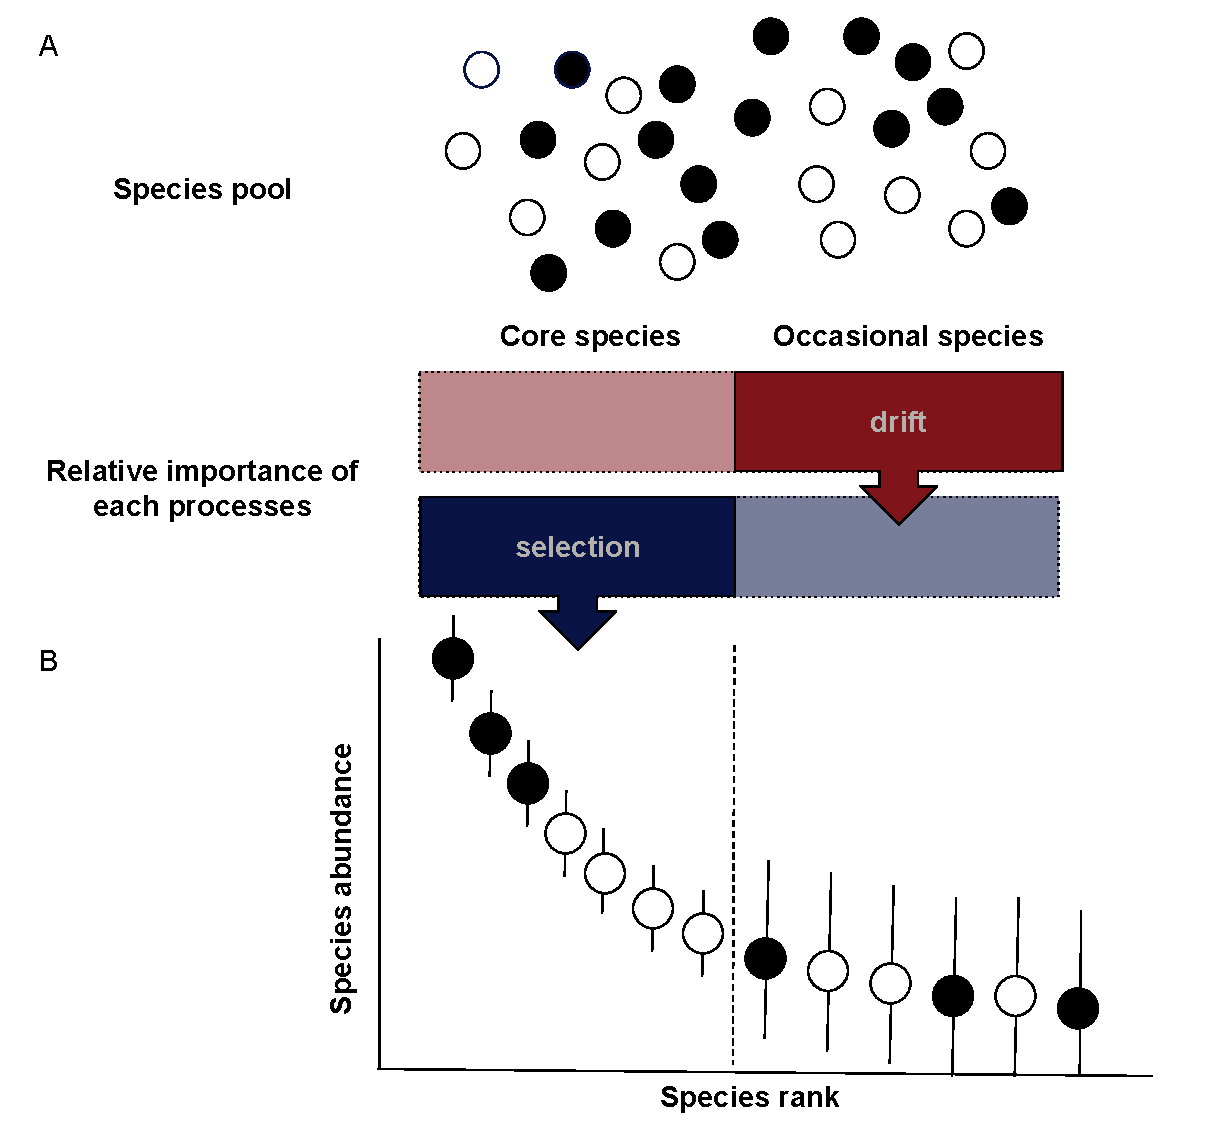
\includegraphics[scale=.48]{fig/figura_conceitual.pdf}
\end{center}
\caption{Interpretation of how niche and neutral processes can generate observed patterns of species abundances on core and occasional species. A. Selection and drift are the main processes affecting which species will occur at a specific metacommunity. Both processes occur at the same time and the relative importance of both can be quantifyied by our modeling approach. B. Core species would be mainly driven by selection processes, resulting in species traits correlated to abundance. Occasional species would be mainly affected by drift, and it would not matter what trait a species have. Remaining variance of mean abundance of each species is due to drift among species sharing the same ecological strategies and limited dispersal among and within metacommunities.} \label{fig:final}
\end{figure}

%\newpage

% including supplementary
\title{Supplementary material}
\author{}
\date{}

\begin{document}
\maketitle



In order to show how we implemented our framework and how model
components are translated into selection and drift dynamics we applied
our approach to simulated communities to address
the following questions:
% performed
% simulations as described below. Our goal is to address main criticisms
% of our framework being:
(1) Are fixed and random effects of our models actually
capturing selection and drift dynamics? (2) Are random effects only
capturing drift dynamics or uninformed species traits are inflating
random effects?


\subsection*{Goals}\label{material-and-methods}
% PI 17 dez 2020: esta seção já me parece metodologia mesmo, e os goasls eriam o que está acima
We use simulated communities assembled by selection and drift dynamics
in order to show how fixed and random effects capture different
ecological processes. Also, we use traits with strong and weak
correlations to species abundance in order to show how fixed and
random effects capture drift dynamics when traits are
uninformative. We thus simulated three scenarios, with the same data
structure as our abundance data of ferns in three mountain chains in
southern Brazil:


\begin{itemize}
\tightlist
\item
  Deterministic community with traits strongly correlated with species abundance from Poisson sample
\item
  Deterministic community with traits poorly correlated with species abundance from Poisson sample
\item
  Stochastic community with traits strongly correlated with species abundance from Poisson sample
\end{itemize}



\subsection*{Building simulated
communities and samples}\label{building-simulated-communities}

We used the R package MCSIM (available at:
\url{https://github.com/sokole/MCSim}) from Eric Sokol to create
simulations of
metacommunities %to test assumptions about their underlying processes underlying
(Sokol et al.~2015). To replicate a data set analogous to our data all
metacommunities were composed by 30 sites in three regions with 153
species. We fixed the total number of individuals in the metacommunity
as 1,000,000 and migration parameter at 0.5.

Deterministic communities
were modelled based on an environmental gradient that weights the
selection of colonizers of each site from a common poll, based on how
well fitted each species is to the environmental conditions of each
site.  In addition, deterministic communities exhibit a flat dispersal
kernel, to express that dipsersal is not limited.  For deterministic
communities with strong traits, we defined values of traits that were
highly correlated with the environmental response of each species to
the environmental gradient.

In stochastic communities species are also selected based on the
environmental gradient, however the standard deviation from the mean
response to the gradient is high enougj to emcompass the whole
gradient.  In practice, such arametrization ensues a neutral scenario
(Sokol et al.~2015). Also, stochastic communities exhibit a limited
dispersal kernel, to simulate dispersal limitaion among sites and more
strongly among regions.

For each scenario we generated 100 communities and then we simulated
Poisson samples from each community to build data sets used in our
model selection framework. Each sample had on avreage 20,000
individuals (that is, 2\% of the total number of individuals).

\subsection*{Fitting models to simulated
data}\label{fitting-models-to-simulated-data}

We used our framework to fit models to the sample abundances of each
community in the three scenarios. We then calculated the proportion of
simulations that resulted in which each each model was well supported
by the data \(\Delta{AIC} < 2\). We also calculated the adjusted
\(R^{2}\) for the selected models, from code adapted from Johnson
(2014), to calculate: (i) marginal and conditional \(R^{2}\) of each
model, (ii) enhanced agreement repeatibility (Stofel et al
2107). Agrrement repeatability can is the ratio of the intra-class
variance for a given random factor and the total variance estimated by
the models, including fixed-effect variances. These functions are
available in the script \texttt{functions.R} accompanying this text, but
applies only to models within our framework. % PI 17 dez 2020:  ao framework ou aos modelos do nosso estduo de caso? Acho que é o segundo caso, não?
For generic functions
please see packages (rptR and MuMIn).

\subsection*{Results}\label{results}

Based on our simulations, we found that samples from deterministic
communities with traits highly correlated to abundance provide strong
support for the models that express the Trait-mediated Selection
hypothesis (Table S1). As expected, samples from deterministic
communities with traits poorly correlated to abundance support mainly
the models that correspond to the Selection \& Drift
hypothesis. Samples from stochastic communities are also strongly
support the model that express the Drift hypothesis.

By examining the partition of $R^{2}$ values, we can understand how
selection and drift terms in the best-supported statistical models
capture variance in species abundance
(Figure S1). When comparing deterministic communities with traits
correlated to abundance with stochastic communities, it is clear that
in the first case, most of the $R^{2}$ is accounted by the fixed
effects. In contrast, the variance in the abundance of stochastic
communities is mostly due to the component of regional limited
dispersal (1|SP:R). For deterministic communities with traits poorly
correlated to abundance, we still see that the largest share of the $R^{2}$ 
is for selection terms. However, most of the variation is 
explained by the term (1 + G|SP) which represents the variance of
species abundance in respect to the gradient but independent of the
measured traits. In other words, this term can identify if the model
is being built with the wrong traits.

\begin{table}[!ht]

\caption{\label{tab:table-prop}Proportion of models with {$\Delta$} AIC {$<$}  2 at each scenario.}
\centering
\begin{tabular}[t]{p{3cm}p{2cm}p{2.cm}p{2.cm}p{2cm}p{2cm}p{2cm}}
\toprule
\textbf{Scenario} & \textbf{Trait-mediated Selection} \& \textbf{Drift} & \textbf{Selection \& Drift} & \textbf{Trait-mediated Selection} & \textbf{Selection \& Drift} & \textbf{Drift} & \textbf{Idyosyncratic}\\
\hline
Deterministic with right traits & 1.00 & 0.00 & 0 & 0.00 & 0 & 0\\
Deterministic with wrong traits & 0.00 & 0.82 & 0 & 0.18 & 0 & 0\\
Stochastic with right traits & 0.02 & 0.00 & 0 & 0.00 & 1 & 0\\
\bottomrule
\end{tabular}
\end{table}

\begin{figure}
\centering
\includegraphics[scale=.9]{fig/S1.png}
\caption{Figure S1.}\label{fig:r2}
\end{figure}

\end{document}



\end{document}




